% Chapter Chapter 2 For Reproducible Research in R and RStudio
% Christopher Gandrud
% Created: 16/07/2012 05:45:03 pm CEST
% Updated: 23 September 2012




\chapter{Getting Started with Reproducible Research}\label{GettingStartedRR}

Researchers often start thinking about making their research reproducible near the end of the research process when they get start writing up the results. Or maybe later, like when a journal has conditioned an article's acceptance on making its data available. Or maybe even later when another researcher asks if they can use the data. By these points there may be numerous versions of the data set and records of the analyses strewn across multiple folders on the researcher's computer. It can be difficult and time consuming to sift through these files to create an accurate account of how the results were reached. Waiting until near the end of the research process to start thinking about reproducibility can lead to incomplete documentation that does not give us an accurate account of how findings were made. Keeping your eye on reproducibility from the beginning of the research process and continuing to follow a few simple guidelines throughout your research can help solve these problems. Remember ``reproducibility is not an afterthought--it is something that must be built into the project from the beginning"\cite[386]{Donoho2010}.

This chapter first gives you a big picture overview of the reproducible research process: a workflow for reproducible research. Then it covers some of the key guidelines that can help make your research more reproducible.

\section{The Big Picture: A workflow for reproducible research}

To make our research accurately reproducible we should start thinking at the beginning--the data gathering stage--about how other researchers and ourselves will be able to reproduce our results. This book teaches the tools for an integrated workflow for reproducible research. It covers tools that we can use across the three basic stages that most computational researchers go through to answer their research questions:

\begin{itemize}
    \item data gathering,
    \item data analysis,
    \item results presentation.
\end{itemize}

Each stage is covered in its own part of the book. Tools for reproducibly gathering data are covered in Part II. Part III teaches tools for tying the data we gathered to our statistical analyses and presenting the results with tables and figures. Part IV discusses how to tie these findings into documents we can use to advertise our findings to others.

If you are like me, you will probably be tempted to start using the individual tools of reproducible research as soon as you find learn them. However, I would recommend stepping back and considering how the stages of reproducible research {\emph{tie}} together. This will make your reproducible research workflow more coherent from the beginning and save you a lot of backtracking later on.  Figure \ref{WorkflowTies} gives you a preview of the workflow and some of the commands we will learn in this book for tying it together. For more information on these tie commands see Table \ref{TableTieCommands}. The tips in this chapter should guide you through the reproducible research workflow. The rest of the book will give you the details.

\clearpage
\thispagestyle{plain}
\begin{landscape}
\begin{figure}[th!]
    \caption{Example Workflow \& Commands to Tie it Together}
    \label{WorkflowTies}
    \begin{center}
    
    %%%%%%%%%%%%%%
% Reproducible research workflow + link commands
% Christopher Gandrud
% Updated 19 November 2012
%%%%%%%%%%%%%%

% Define colors for figure
%% Color palette (GnBU) chosen using ColorBrewer 2.0
%% See: http://colorbrewer2.org/
%% Not used in the print version
\definecolor{Blue}{HTML}{7BCCC4}
\definecolor{LiteBlue}{HTML}{A8DDB5}
\definecolor{DarkBlue}{HTML}{08589E}

\definecolor{GrayLine}{HTML}{BDBDBD}

% Set node styles
%% Workflow stage nodes
\tikzstyle{Stage} = [draw=Blue, 
                     %fill=Blue, 
                     rectangle, 
                     text width=7em, 
                     inner sep=0.5cm, 
                     font=\small]

% Raw Data nodes
\tikzstyle{RawData} = [draw=LiteBlue, 
                       %fill=LiteBlue, 
                       decorate,
                       decoration={random steps,
                                   segment length=2pt,
                                   amplitude=2pt},
                       inner sep=0.25cm, 
                       font=\scriptsize]
                    
% Separator line style
\tikzstyle{sepline} = [draw,
                        very thick,
                        color=GrayLine]
                        
% Link command nodes       
\tikzstyle{Links} = [draw=none, 
                          text width=6em,
                          text=DarkBlue,
                          font=\small]

% Begin tikz picture
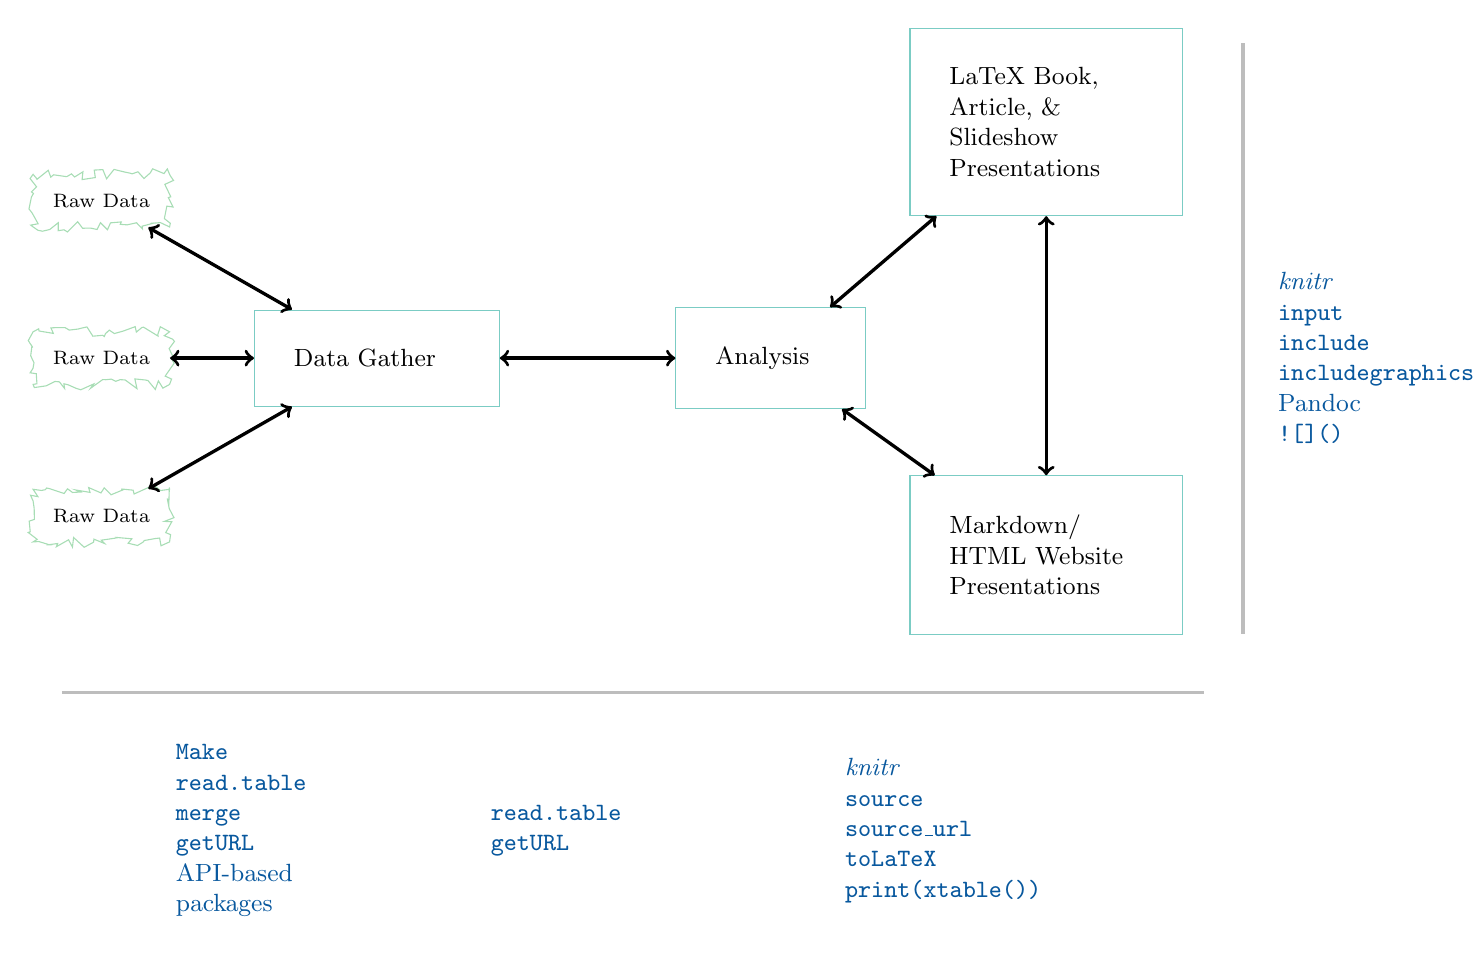
\begin{tikzpicture}

    % Raw Data Nodes
    \node (Data1) at (-3, 7) [RawData]{Raw Data};
    \node (Data2) at (-3, 5) [RawData]{Raw Data};
    \node (Data3) at (-3, 3) [RawData]{Raw Data}; 
    
    % Workflow stage nodes
    \node (DataGather) at (0.5, 5) [Stage, text width= 6em]{Data Gather};
    \node (Analysis) at (5.5, 5) [Stage, text width= 4em]{Analysis};
    \node (Presentation1) at (9, 8) [Stage]{LaTeX Book, \\ Article, \& \\ Slideshow \\ Presentations};
    \node (Presentation2) at (9, 2.5) [Stage]{Markdown/ \\ HTML Website \\ Presentations};

    % Lines
    \draw [<->, very thick] (Data1) -- (DataGather);
    \draw [<->, very thick] (Data2) -- (DataGather);
    \draw [<->, very thick] (Data3) -- (DataGather);
    \draw [<->, very thick] (DataGather) -- (Analysis);
    \draw [<->, very thick] (Analysis) -- (Presentation1);
    \draw [<->, very thick] (Analysis) -- (Presentation2);
    
    \draw [<->, very thick] (Presentation1) -- (Presentation2);
    
    \path [sepline] (-3.5, 0.75) -- (11, 0.75);
    \path [sepline] (11.5, 9) -- (11.5, 1.5);
    
    % Link command nodes
 
    \node (pres) at (13, 5) [Links]{{\emph{knitr}} \\ \texttt{input} \\ \texttt{include} \\ \texttt{includegraphics} \\ Pandoc \\ \texttt{![]()}};
    \node (knitr) at (7.5, -1) [Links]{ {\emph{knitr}} \\ \texttt{source} \\ \texttt{source\_url} \\ \texttt{toLaTeX} \\ \texttt{print(xtable())} };
    \node (readData) at (3, -1) [Links]{ \texttt{read.table} \\ \texttt{getURL} };
    
    \node (importData) at (-1, -1) [Links]{ \texttt{Make} \\ \texttt{read.table} \\ \texttt{merge}\\ \texttt{getURL} \\ API-based packages };

  
\end{tikzpicture}
    \end{center}
\end{figure}
\end{landscape}

\subsection{Reproducible Theory}

An important part of the research process that I do not actively discuss in this book is the theoretical stage. Ideally, if you are using a deductive research design, the bulk of this work would precede and even guide the data gathering process. Because I don't cover this stage of the research process doesn't mean that theory building shouldn't be reproducible. It can in fact be ``the easiest part to make reproducible" \cite[1254]{Vandewalle2007}. For mathematically based theory results clear and complete descriptions of the proofs should be given. Quotes and paraphrases from previous works in the literature obviously need to be fully cited so that others can verify that they accurately reflect the source material.

Just because I don't cover theory replication in depth in this book, doesn't mean that you can't find out information about it here. I do touch on some of the ways to incorporate proofs and citations into your presentation documents. These tools are covered in Part IV.

\section{Practical tips for reproducible research}

Before we start learning the details of reproducible research with R and RStudio it is useful to cover a few broad tips that will help us organize our research process and put these skills in perspective. The tips are:

\begin{enumerate}
    \item Document everything!,
    \item Everything is a file,
    \item All files should be human readable,
    \item Reproducible research projects are many files explicitly tied together,
    \item Don't put too much in one file
    \item Have a plan to organize, store, and make your files available.    
\end{enumerate}

\noindent Using these tips will help make your computational research really reproducible.

\subsection{Document everything!}

In order to reproduce your research others must be able to know what you did. You have to tell them what you did by documenting as much of your research process as possible. Ideally, you should tell your readers how you gathered your data, analyzed it, and presented the results.

One important part of documenting everything with R is to \emph{record your session info\index{session info}}. Many things in R stay the same over time, which makes it easy for future researchers to recreate what was done in the past. However, things--syntax in particular--do can change from one version of R to another. Also, the way R functions may be handled slightly different on different operating systems. Finally, you may have R set to load packages by default. These packages might be necessary to run your code, but other people might not be able know what packages were loaded from just looking at your source code. The \texttt{sessionInfo} command prints a record of all of these things. The information from the session I used to create this book is:

\begin{knitrout}
\definecolor{shadecolor}{rgb}{0.969, 0.969, 0.969}\color{fgcolor}\begin{kframe}
\begin{alltt}
\hlfunctioncall{sessionInfo}()
\end{alltt}
\begin{verbatim}
## R version 2.15.1 (2012-06-22)
## Platform: x86_64-apple-darwin9.8.0/x86_64 (64-bit)
## 
## locale:
## [1] C/en_US.UTF-8/C/C/C/C
## 
## attached base packages:
## [1] tools     stats     graphics  grDevices utils    
## [6] datasets  methods   base     
## 
## other attached packages:
##  [1] reshape_0.8.4       plyr_1.7.1         
##  [3] MCMCpack_1.2-4      coda_0.15-2        
##  [5] lattice_0.20-10     Zelig_3.5.5        
##  [7] boot_1.3-5          MASS_7.3-21        
##  [9] xtable_1.7-0        texreg_1.02        
## [11] openair_0.7-0       markdown_0.5.2     
## [13] knitcitations_0.1-0 bibtex_0.3-2       
## [15] knitr_0.8           ggplot2_0.9.2.1    
## [17] extrafont_0.11      devtools_0.8       
## [19] apsrtable_0.8-8    
## 
## loaded via a namespace (and not attached):
##  [1] Matrix_1.0-9       RColorBrewer_1.0-5
##  [3] RCurl_1.91-1       Rttf2pt1_1.1      
##  [5] XML_3.9-4          cluster_1.14.2    
##  [7] codetools_0.2-8    colorspace_1.1-1  
##  [9] dichromat_1.2-4    digest_0.5.2      
## [11] evaluate_0.4.2     formatR_0.6       
## [13] grid_2.15.1        gtable_0.1.1      
## [15] httr_0.1.1         labeling_0.1      
## [17] memoise_0.1        mgcv_1.7-21       
## [19] munsell_0.4        nlme_3.1-104      
## [21] parallel_2.15.1    pkgmaker_0.8      
## [23] proto_0.3-9.2      reshape2_1.2.1    
## [25] scales_0.2.2       stringr_0.6.1     
## [27] whisker_0.3-1
\end{verbatim}
\end{kframe}
\end{knitrout}


\noindent It is good practice to include make output of the session info available either in the main document or in a separate readme\index{README file} file. If you want to nicely format the information for a \LaTeX document simply use the {\tt{toLatex}} command.

\begin{knitrout}
\definecolor{shadecolor}{rgb}{0.969, 0.969, 0.969}\color{fgcolor}\begin{kframe}
\begin{alltt}
\hlfunctioncall{toLatex}(\hlfunctioncall{sessionInfo}())
\end{alltt}
\end{kframe}
\end{knitrout}


\noindent Chapter \ref{DirectoriesChapter} gives specific details about how to create readme files with dynamically included session information.

\subsection{Everything is a (text) file}

Your documentation is stored in files that include data, analysis code, the write up of results, and explanations of these files (e.g. data set codebooks, session info files, and so on). Ideally, you should use the simplest file format possible to store this information. Usually the simplest file format is the the humble, but versatile, text file is the simplest file format.\footnote{Depending on the size of your data set it may not be feasible to store it as a text file. Nonetheless, text files can still be used for analysis code and presentation files.} 

Text files are extremely nimble. They can hold data in, for example, comma-separated values {\tt{.csv}} \index{comma-separated values6} files. They can contain our analysis code in {\tt{.R}} files. And they can be the basis for our presentation documents as markup documents like {\tt{.tex}} or {\tt{.md}}, for \LaTeX and Markdown files respectively. All of these files can be opened by any program that can read text files--i.e. files with the generic file extension {\tt{.txt}}. 

The main reason reproducible research is best stored in text files is that this helps {\bf{future proof}} our research. Other common file formats, like Microsoft Word \index{Microsoft Word} or Excel \index{Microsoft Excel} documents change regularly and may not be compatible with future versions of these programs. Text files, on the other hand, can be opened by a very wide range past and, more likely than not, future programs. Even if future researchers do not have R or a \LaTeX distribution, they will still be able to open our text files and, aided by frequent comments, be able to understand how we conducted our research \cite[3]{Bowers2011}.

Text files are also very easy to search and manipulate with a wide range of programs--such as R--that can find and replace text characters as well as merge and separate files. They have a number of clear benefits for reproducible research including enabling versioning and track changes in programs such as Git (see Chapter \ref{Storing}).   

\subsection{All files should be human readable}

Treat all of your research files as if someone who has not worked on the project will try to read them and understand them. Computer code is a way of communicating with the computer. It is `machine readable' in that the computer is able to use it to understand what we want done.\footnote{Of course, if it does not understand it will usually give us an error message.} Hopefully, the researcher understands what they are communicating when they write their code. However, there is a very good chance that other people (or you six months in the future) will not understand what is being communicated. So, you need to make your documentation `human readable'. To make your documentation accessible to other people you need to {\bf{comment frequently}} \cite[3]{Bowers2011} and {\bf{format your code using a style guide}} \cite[]{Nagler1995}. For especially important piece of code you should use {\bf{literate programming}}--where the code and the presentation document text appear in the same document--so that it is very clear to others how you accomplished a piece of research.

\paragraph{Commenting}
In R everything on a line after a {\tt{\#}} hash (number) character is ignored by R, but is readable to people who open the file. The hash character is a comment declaration\index{comment declaration} character. You can use the {\tt{\#}} to place comments telling other people what you are doing. Here are some examples:

\begin{knitrout}
\definecolor{shadecolor}{rgb}{0.969, 0.969, 0.969}\color{fgcolor}\begin{kframe}
\begin{alltt}
\hlcomment{# A complete comment line}
2 + 2  \hlcomment{# A comment after R code}
\end{alltt}
\begin{verbatim}
## [1] 4
\end{verbatim}
\end{kframe}
\end{knitrout}


Because on the first line the {\tt{\#}} is placed at the very beginning, the entire line is treated as a comment. On the second line the {\tt{\#}} is placed after the simple equation {\tt{2 + 2}}. R runs the equation as usual and fines the answer {\tt{4}}, but it ignores all of the words after the hash. 

According to Nagler \citeyearpar[491]{Nagler} to make your code understandable it is good practice to:

\begin{itemize}
    \item write a comment before a block of code describing what the code does,
    \item comment on any line of code that is ambiguous.
\end{itemize}

\noindent In this book I follow these guidelines when displaying written code. 

Different languages have different comment declaration characters. In \LaTeX everything after the {\tt{\%}} percent sign is treated as a comment and in markdown/HTML comments are placed inside of {\tt{\textless !-- --\textgreater}}. The hash character is used for comment declaration in shell scripts.

All of your source code files should begin with a comment header that {\emph{at the least}} should include:

\begin{itemize}
    \item a description of what the file does,
    \item the date it was last updated,
    \item the name of the file's creator and any other contributors
\end{itemize}

\noindent You may also want to include other information in the header such as what other files it depends on, what output files it produces, and what version of the programming language you are using. 

Here is an example file header for an R source code file that creates the third figure in an article titled ``My Article":

\begin{knitrout}
\definecolor{shadecolor}{rgb}{0.969, 0.969, 0.969}\color{fgcolor}\begin{kframe}
\begin{alltt}
\hlcomment{##################}
\hlcomment{# Source code file used to create Figure 3 in \hlstring{''}My Article\hlstring{''}}
\hlcomment{# Created by Christopher Gandrud}
\hlcomment{# Updated 21 September 2012}
\hlcomment{##################}
\end{alltt}
\end{kframe}
\end{knitrout}


\noindent Feel free to use things like the long series of hash marks above and below the header, white space, and indentations to make your comments more readable. 

\paragraph{Style guides}
In natural language writing you don't necessarily need to follow a \index{style guide} for things such as punctuation. People could probably figure out what you are saying. But it would be a lot easier for your readers if you use consistent rules. The same is true when writing R code. It's good to follow consistent rules for formatting your code so that:

\begin{itemize}
    \item it's easier for others to understand,
    \item it's easier for you to understand.
\end{itemize}

There are a number of R style guides. Most of them are similar to the Google R Style Guide \index{Google R Style Guide} (\url{http://google-styleguide.googlecode.com/svn/trunk/google-r-style.html}). Hadley Wickham \index{Hadley Wickham} has a nicely presented style guide. You can find it at \url{https://github.com/hadley/devtools/wiki/Style}. You can also use the {\tt{formatR}} \index{\tt{formatR}} package to automatically reformat your code so that it is easier to read.

\paragraph{Literate programming}

For particularly important pieces of research code it may be useful to not only comment on the source file, but also display code in presentation text. For example, you may want to include key parts of the code you used for your statistical model and an explanation of this code in an appendix following your article. This is commonly referred to as literate programming \index{literate programming} \cite[]{Knuth1992}. This book teaches you how to use the {\emph{knitr}} package, a very useful tool for literate programming. 

\subsection{Reproducible research projects are many files explicitly tied together}

If everything is just a text file then research projects can be thought of as individual text files that have a relationship with one another. A data file is used as input for an analysis file. The results of an analysis are shown and discussed in a markup file that is used to create a slideshow or PDF document. Researchers often do not explicitly document the relationships between files that they used in their research. For example, the results of an analysis--a table or figure--may be copied and pasted into a presentation document. It will be very difficult for future researchers to trace the results table or figure back to a particular analysis and a particular data set. Therefore, it is important to make the links between your files explicit. 

The most dynamic way to do this is to explicitly link your files together using what I'll call {\bf{tie commands}}. \index{tie commands} These commands instruct the computer program you are using to gather data, run an analysis, or compile a presentation document to use information from another file. I have compiled a selection of tie commands used in this book in Table \ref{TableTieCommands}.

\subsection{Don't put too much in one file}

Files that contain many different operations can be very difficult to navigate, even if they have detailed comments. For example, it would be very difficult to find any particular operation in a file that had the code used to gather all of the data and manipulate the data, run all of the statistical models, and create the results figures and tables. If you have a hard time finding things in a file you created, think of the difficulties independent researchers will have! 

Because we have so many ways to link files together there is really no need to lump many different operations into one file. So, we can make our operations modular. One source code file should to one task. This will make your code easier to read. By breaking your operations into discrete chunks, it will also make it easier for you and others to find errors \cite[490]{Nagler1995}.  

\begin{landscape}
\begin{table}
    \caption{A Selection of Commands for Tying Together Your Research Files}
    \label{TableTieCommands}
    \vspace{0.3cm}
    {\small{
    \begin{tabular}{l c p{6.5cm} c}
        \hline \vspace{0.15cm}
        Command/Package & Language & Description & Chapters for Further Information \\[0.3cm]  
        \hline \hline
        {\emph{knitr}} & R & R package with commands for tying commands from R and other programming languages commands into presentation documents & Discussed throughout the book \\[0.25cm]
        {\tt{read.table}} & R & Reads a table into R. You can use this to import plain-text file formated data into R. & \ref{DataGather} \\[0.25cm]
        {\tt{read.csv}} & R & Same as \texttt{read.table} with default arguments set to import \texttt{.csv} formatted data files. & \ref{DataGather} \\[0.25cm]  
        API-based packages & R & Various packages use APIs to gather data from the internet. & \ref{DataGather} \\[0.25cm]
        {\tt{merge}} & R & Merges together data frames. & \ref{DataClean} \\[0.25cm]
        {\tt{source}} & R & Runs an R source code file & \ref{StatsModel} \\[0.25cm]
        {\tt{source\_url}} & R & From the {\emph{devtools}} package. Runs an R source code file from a secure ({\tt{https}}) url like those used by GitHub & \ref{StatsModel} \\[0.25cm]
        {\tt{print(xtable())}} & R & Combining the \texttt{print} \& \texttt{xtable} commands creates \LaTeX \& HTML tables from R objects & \ref{TablesChapter} \\[0.25cm]
        {\tt{toLaTeX}} & R & Converts R objects to \LaTeX & \ref{GettingStartedRR} \\[0.25cm]
        {\tt{input}} & \LaTeX & Includes \LaTeX files inside of other \LaTeX files & \ref{LargeDocs} \\[0.25cm]
        {\tt{include}} & \LaTeX & Similar to {\tt{input}}, but puts page breaks on either side of the included text. Usually this it is used for including chapters chapters. & \ref{LargeDocs} \\[0.25cm]
        {\tt{includegraphics}} & \LaTeX & Inserts a figure into a \LaTeX document. & \ref{FiguresChapter} \\[0.25cm]
        \texttt{![]()} & Markdown & Inserts a figure into a Markdown document. & \ref{MarkdownChapter} \\  [0.25cm]      
        \hline 
    
    \end{tabular}
    }}
\end{table}
\end{landscape}

\subsection{Have a plan to organize, store, and make your files available}

Finally, in order for independent researchers to reproduce your research they need to be able actually access the files that instruct them how to do this. Files also need to be organized so that independent researchers can figure out how they fit together. So from the beginning of your research process you should have a plan for organizing your files and a way to make them accessible. Chapter \ref{DirectoriesChapter} discusses file organization in detail. Chapter \ref{Storing} teaches you a number of ways to make your files accessible through cloud computing services like Dropbox\index{Dropbox} and GitHub\index{GitHub}. 
